\chapter{Практическая часть}
\label{ch:practice}
\linespread{1.5}
\section{Выгрузка, обработка и агрегация исходных данных}

Все исходные данные, включая статистику заболеваемости ВИЧ-инфекцией, а также дополнительную статистику по выбранным социально-демографическим факторам, были выгружены с порталов ЕМИСС и Роспотребнадзора в формате csv-таблиц. Для решения поставленной задачи машинного обучения необходимо объединить все собранные таблицы воедино таким образом, чтобы для каждого субъекта Российской Федерации была отражена ежегодная статистика по всем собранным данным. Стоит отметить, информация о заболеваемости ВИЧ-инфекцией доступна в период с 1999 года по 2022 год, все прочие факторы будут приведены к этому интервалу. Перед объединением каждая из таблиц прошла процедуру предобработки, которая включала в себя несколько этапов:

\begin{enumerate}
	\item Таблица проверена на наличие дублирующихся строк, при наличии таковых все вторичные строки были удалены.
	
	\item Таблица проверена на наличие аномальных значений (ошибок в данных). Так, например, в некоторых таблицах вместо численных значений встречались обрывки строк, не несущие полезной информации. Кроме того, в некоторых таблицах встречались недостоверные значения статистики: так, например, на протяжении долгого периода времени уровень безработицы в Чеченской Республике оставался нулевым. Подобные аномалии были устранены, все недостоверные значения статистики заменены пропусками.
	
	\item Наименования территорий, используемые в таблице, были приведены к единому стандарту. Изначально в разных таблицах встречаются варьирующиеся наименования одних и тех же территорий (пр. <<Ямало-Ненецкий автономный округ>> и <<Ямало-Ненецкий АО>>).
	
\end{enumerate}

Для таблицы, содержащей распределение новых случаев ВИЧ между группами риска, помимо стандартной процедуры предобработки была также проведена процедура извлечения полезных признаков. Таблица содержит в себе данные о количестве проведенных тестов на наличие ВИЧ (столбец <<ИФА>>), и числе положительных результатов (столбец <<ИБ>>), для каждой из категорий населения, указанных с помощью кодов (столбец <<Код>>). Фрагмент данной таблицы с расшифровкой кодов приведен в таблице \ref{tab:f4_table}.

% Please add the following required packages to your document preamble:
% \usepackage{graphicx}
\begin{table}[h]
	\caption{Фрагмент таблицы ВИЧ-контингентов}
	\label{tab:f4_table}
	\resizebox{\textwidth}{!}{%
		\begin{tabular}{|l|l|l|l|l|}
			\hline
			\textbf{Год} & \textbf{Код}                        & \textbf{Территория} & \textbf{ИФА} & \textbf{ИБ} \\ \hline
			2008         & Потребители инъекционных наркотиков & Алтайский край      & 7788         & 650         \\
			2008         & МСМ                                 & Алтайский край      & 5            & 0           \\
			2008         & Больные ЗППП                        & Алтайский край      & 12921        & 107         \\
			2008         & Обследованные доноры                & Алтайский край      & 106088       & 48          \\ \hline
		\end{tabular}%
	}
\end{table}

Пользуясь данной информацией, мы извлекаем 2 полезных знания, которые могут помочь в предсказании заболеваемости:
\begin{enumerate}
	\item Отношение числа инфицированных ("ИБ") к числу обследованных ("ИФА") для каждой из категорий населения. Данное отношение показывает, насколько высок риск заражения внутри каждой группы. 
	
	\item Доля инфицированных лиц ("ИБ") по каждой категории относительно общего количества инфицированных. Данный показатель отражает, какая из групп является ведущей в распространении заболевания.
\end{enumerate}


Стоит отметить, что подавляющее число проведенных тестов и положительных результатов принадлежат основным 5-6 группам риска, все остальные группы малочисленны (доля числа инфицированных <1 \%) и были объединены в <<Прочие контингенты>>. Распределение общего числа инфицированных лиц по группам приведено на рисунке \ref{fig:f4_fractions}.

\newpage
\begin{figure}[ht]
	\centering
	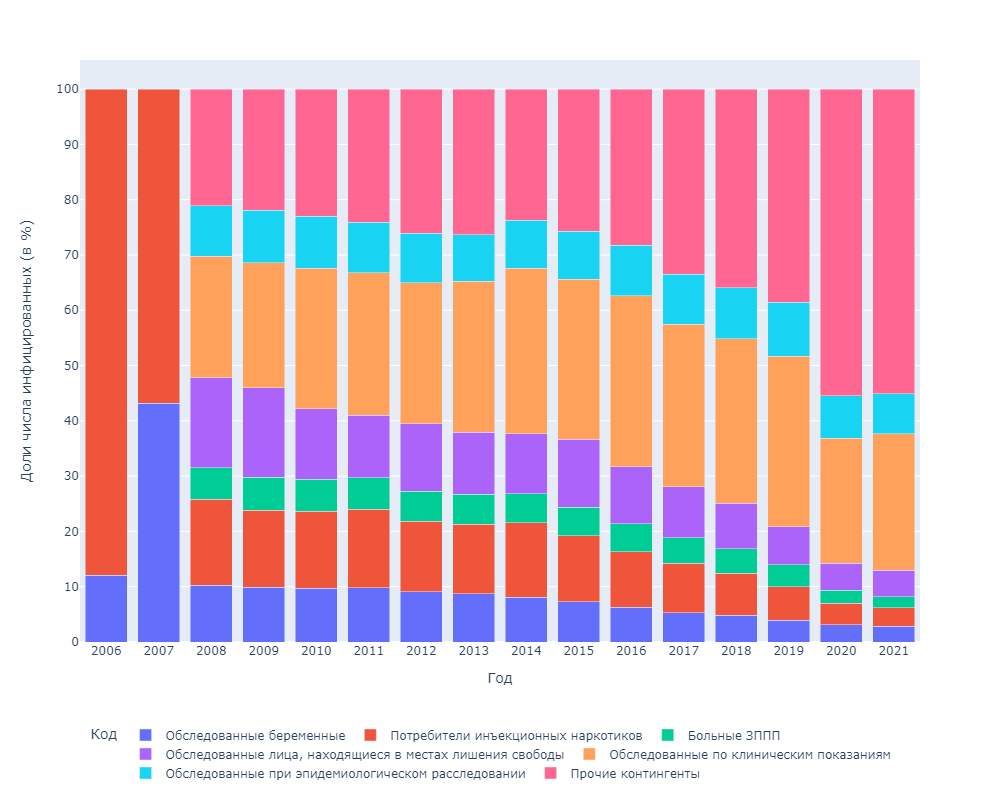
\includegraphics[width=1\textwidth]{f4_fractions}
	\caption{Распределение числа инфицированных по группам}
	\label{fig:f4_fractions}
\end{figure}

После прохождения процедур предобработки, все таблицы были соединены воедино, полученный результат и будет подаваться на вход модели машинного обучения. Всего в финальной таблице отражено 83 субъекта Российской Федерации, 34 социально-демографических предиктора и 2 целевые статистики: число новых случаев ВИЧ (НС), и уровень заболеваемости ВИЧ-инфекцией в просантимилле (НС \%).

Обратим внимание на то, что каждая из исходных таблиц содержала данные за разные промежутки времени, поэтому в результате их слияния было получено большое количество пропущенных значений. Проиллюстрируем количество колонок, имеющих в себе пропущенные значения, на рисунке \ref{fig:f4_missing}.
\newpage
\begin{figure}[ht]
	\centering
	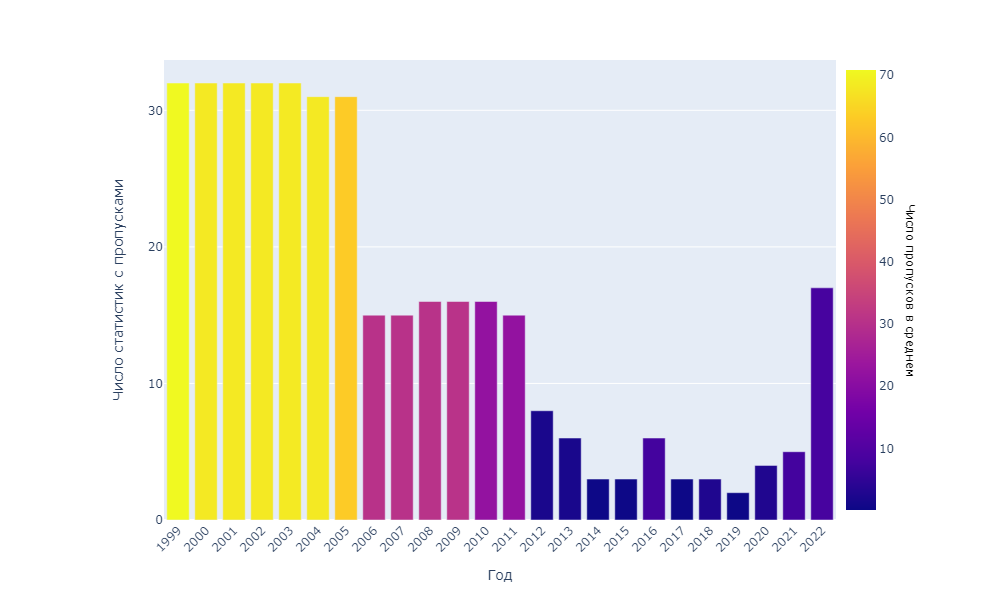
\includegraphics[width=1\textwidth]{missing_values_plot}
	\caption{Количество отсутствующих предикторов по годам}
	\label{fig:f4_missing}
\end{figure}


Как видно из графика, до 2005го года включительно большинство социально-демографических предикторов имеет очень большое количество пропусков. Начиная с 2006го года ситуация значительно улучшается, колонок с пропусками становится меньше, и в среднем число пропусков в каждой из них уменьшается вдвое. Кроме того, в 2022ом году статистика о заболеваемости ВИЧ-инфекцией на момент рассмотрения доступна лишь по малой части из субъектов. Учитывая эти факты, все наличные временные ряды будут рассмотрены в промежутке от 2006го до 2021 года включительно.

Для заполнения оставшихся пропусков были апробированы несколько методов:
\begin{itemize}
	\item заполнение предыдущим значением временного ряда;
	\item заполнение следующим значением временного ряда;
	\item заполнение пропущенных признаков с помощью линейной регрессии относительно наличных признаков.

\end{itemize}
 
 Как показали дальнейшие испытания, в целом качество предсказания всех моделей было выше в случае использования линейной регрессии, которая была реализована с применением класса <<Iterative Imputer>> из библиотеки <<scikit-learn>>.
 
\section{Описание используемых методов предсказания}

Для решения поставленной задачи машинного обучения были выбраны две наиболее перспективные нейросетевые архитектуры:

\begin{itemize}
	
	\item архитектура MES-LSTM, представляющая из себя комбинацию двойного экспоненциального сглаживания и рекуррентной нейронной сети;
	
	\item классическая рекуррентная архитектура LSTM без использования экспоненциального сглаживания.
	
\end{itemize} 

Для оценки эффективности использования нейросетевых моделей в сравнение также были добавлены классические статистические методы предсказания:
 
\begin{itemize}

	\item метод предсказания многомерных временных рядов VARMAX;
	
	\item метод предсказания одномерных временных рядов ARIMA.

\end{itemize}    

Опишем подробнее архитектуру MES-LSTM, представленную в 2021 году \cite{MES_RNN}. Структурная схема модели из оригинальной работы приведена на рисунке \ref{fig:MES_LSTM}.

\begin{figure}[h!]
	\centering
	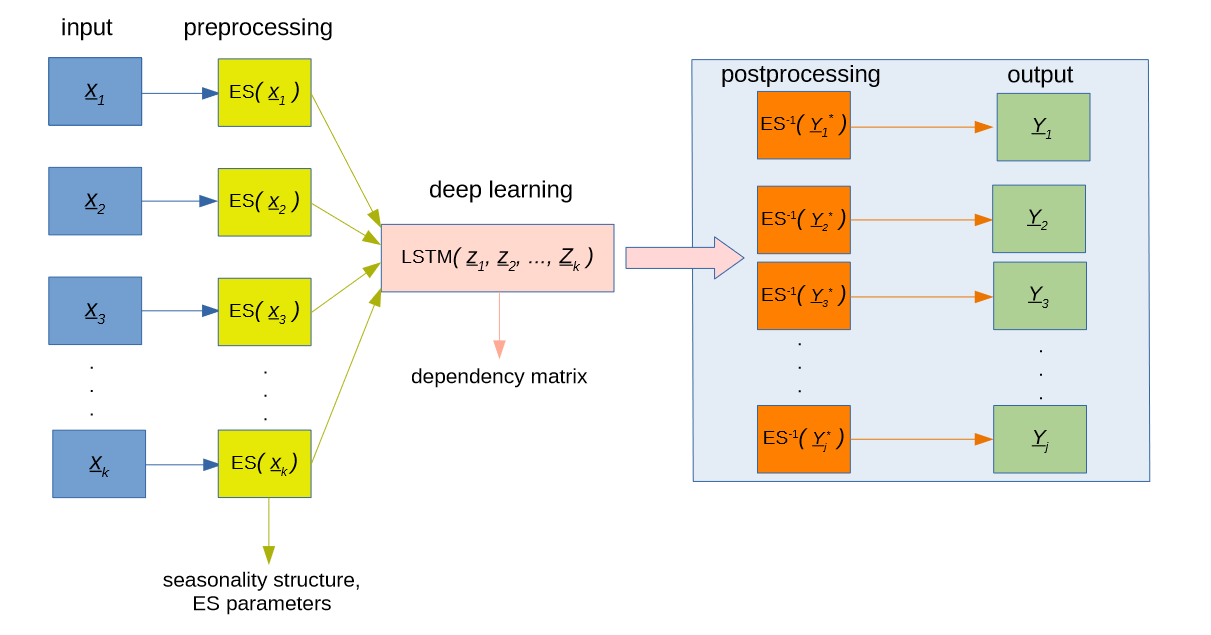
\includegraphics[width=0.9\textwidth]{MES_LSTM}
	\caption{Структурная схема модели MES-LSTM  \\
		Источник: [Mathonsi T., Zyl T.L. van. A Statistics and Deep Learning Hybrid Method for Multivariate Time Series Forecasting and Mortality Modeling  Forecasting. — 2022. — Mar. — Vol. 4, no. 11. — P. 1–25.]}
	\label{fig:MES_LSTM}
	
\end{figure}


\subsection{Слой предобработки (экспоненциальное сглаживание)}
Очищенные и масштабированные данные проходят через слой двойного экспоненциального сглаживания, где с помощью метода метода Хольта для каждой из временных последовательностей извлекается значения уровня и компоненты тренда. Пусть $y_t$ - фактическое значение временного ряда в момент времени $t$. Тогда каждое из значений $y_t$ может быть описано уравнением:

\begin{equation}
	\label{eq:LT_decompose}
	y_t=l_t + b_t + \epsilon_t,
\end{equation}
	

где $l_t$ - значение уровня в момент времени $t$;

 $b_t$ - значение тренда в момент времени $t$;
 
 $\epsilon_t$ - случайный шум с нулевым средним значением и постоянной дисперсией. 
 
Таким образом, в каждый момент времени текущее значение временного ряда складывается из некоторого базового значения (уровня), к которому прибавляется значение тренда (восходящего или нисходящего) и случайная величина ошибки.

Отметим, что в оригинальной работе и в задачах о прогнозировании временного ряда гораздо чаще используется тройное экспоненциальное сглаживание, позволяющее помимо тренда учитывать также сезонность (периодически повторяющиеся паттерны) в данных. Наши временные ряды, однако, представляются слишком короткими и имеют годичную периодичность, поэтому для сглаживания была выбрана упрощенная модель.

Для обучения алгоритма необходимо итеративно вычислить значения уровня и тренда для каждого момента времени, с помощью следующих уравнений:

\begin{equation}
	l_t = \alpha y_t + (1 - \alpha)(l_{t-1} + b_{t-1}),
\end{equation}

где $l_t$ - значения уровня в момент времени $t$;

	$\alpha$ - фактор сглаживания для уровня (0 ≤ $\alpha$ ≤ 1); 
	
	$y_t$ - фактическое значение временного ряда в момент времени $t$; 
	
	$l_{t-1}$ - значение уровня в предыдущий момент времени $t-1$;
	
	$b_{t-1}$ - значение тренда в предыдущий момент времени $t-1$.


 Коэффициент $\alpha$  определяет вес, придаваемый текущей точке данных ($y_t$) по сравнению с предыдущим сглаженным уровнем ($l_{t−1}$) и трендом ($b_{t-1}$). Более высокое значение $\alpha$ приводит к более быстрой реакции на изменения в фактических данных, то есть менее плавному сглаживанию.

\begin{equation}
	b_t = \gamma (l_t - l_{t-1}) + (1 - \gamma) b_{t-1},
\end{equation}
	
где $b_t$ - значение тренда в момент времени $t$; 

$\gamma$ - фактор сглаживания для тренда (0 ≤ $\gamma$ ≤ 1);

$l_t$ - значение уровня в момент времени $t$;

$l_{t-1}$  - значение уровня в предыдущий момент времени $t-1$;

$b_{t-1}$ - значение тренда в предыдущий момент времени $t-1$.

 
 Коэффициент $\gamma$ определяет вес, придаваемый изменению сглаженного уровня ($l_t - l_{t-1}$) по сравнению с предыдущим значением тренда ($b_{t-1}$). Более высокое значение коэффициента приводит к более быстрой реакции на изменение уровня, и, как следствие, более резкой смене тренда.
 
 
Начальные значения параметров инициализируются в модели следующим образом:

\begin{itemize}
	\item начальное значение уровня ($l_1$) приравнивается к первой точке во временной серии ($y_1$);
	
	\item начальный тренд равен нулю.
	
\end{itemize}

В процессе обучения коэффициенты $\alpha, \gamma$, а также начальные значения уровней $l_1, b_1$ выбираются наиболее оптимальным образом с помощью метода максимального правдоподобия. Когда процесс обучения завершен, для получения прогноза необходимо воспользоваться соотношением:

\begin{equation}
	\label{eq:forecasting_Holt}
	\hat{y}_{t+1} = l_t + b_t, 
\end{equation}

​где ​$\hat{y}_{t+1}$ - предсказанное значение ряда для следующего момента времени;

$l_t$ - значение уровня в момент времени $t$;

$b_t$ - значение тренда в момент времени $t$. 

Таким образом, прогноз на следующий период времени ($t+1$) - это сумма значений текущего уровня и текущего тренда.

В нашей модели, однако, экспоненциальное сглаживание не используется напрямую для получения предсказания в следующие моменты времени. Вместо этого, при помощи формулы (\ref{eq:LT_decompose}), из временного ряда извлекаются значения тренда каждой временной последовательности, на основе которых нейросеть LSTM архитектуры строит предсказания. 

Преобразованные временные ряды вместе формируют общую матрицу признаков $X$. Для получения предсказания используется не вся матрица признаков, а только несколько наиболее актуальных значений (так называемое окно обучения). Итоговое уравнение для получения предсказания нашей модели выглядит следующим образом:

\begin{equation}
	\label{eq:forecasting_MESRNN}
	\hat{y}_{t+1} = l_t + RNN(X_{t-size:t, k}),
\end{equation}


где $\hat{y}_{t+1}$ - предсказанное значение;

$l_t$ - значение уровня в момент $t$;

$RNN(X_{t-size:t, k})$ - предсказанное нейросетью значение тренда для момента времени $t$;

$X_{t-size:t, k}$ - срез наиболее актуальных значений матрицы $X$;

$size$ - размер окна обучения;

$k$ - количество предикторов.


\subsection{LSTM слой}

Матрица $X$, полученная на предыдущем шаге и содержащая значения трендов для каждой из временных последовательностей, итеративно, последовательностями по 3 наблюдения ($X_{t-size:t, k}$), подается на вход рекуррентной нейронной сети. Результатом работы модели является предсказанное значения тренда для уровня заболеваемости ВИЧ на текущий год ($\hat{b}_{t}$). 

Нейронная сеть включает в себя три слоя:
\begin{itemize}
	\item входной слой размерности (1, 3, $k$), где $k$ - количество предикторов в модели;
	\item скрытый LSTM слой, состоящий из 50ти нейронов;
	\item выходной слой типа DenseFlipout, позволяющий в процессе обучения получать оптимальное распределение весов для оценки границ доверительного интервала прогнозирования.
\end{itemize}

Структурное описание архитектуры нейросети, использованной для моделей LSTM и MES-LSTM, приведено в таблице \ref{tab:NN_Summary}. 

\begin{table}[ht]
	\caption{Структурная схема нейросети  }
	\label{tab:NN_Summary}
	\resizebox{\textwidth}{!}{%
		\begin{tabular}{lll}
			\hline
			Layer (type)                  & Output Shape                & Param \#                  \\ \hline
			lstm (LSTM)                   & \multicolumn{1}{c}{(1, 50)} & \multicolumn{1}{c}{17000} \\ \hline
			dense\_flipout (DenseFlipout) & \multicolumn{1}{c}{(1,2)}   & \multicolumn{1}{c}{202}   \\ \hline
			Total params: 17, 202         &                             &                           \\
			Trainable params: 17, 202     &                             &                           \\ \hline
			Non-trainable params: 0       &                             &                          
		\end{tabular}%
	}
\end{table}


\subsection{Процедура, обратная к сглаживанию}

Предсказанные на предыдущем этапе значения тренда заболеваемости ВИЧ складываются с извлеченными при сглаживании значениями уровня, в результате чего при помощи формулы (\ref{eq:forecasting_MESRNN}) получается предсказание на следующий момент времени. Таким образом, вместо использования значений локального линейного тренда $b_t$, который фигурирует в формуле для двойного экспоненциального сглаживания (\ref{eq:forecasting_Holt}), мы используем сложные значения нелинейного тренда, предсказанные нейросетью, которые призваны точнее описывать тенденции изучаемого временного ряда.

\section{Метрики оценки качества предсказания}

Для оценки качества предсказания были выбраны метрики MAPE и RMSE, определяемые с помощью формул:

\begin{equation}
	\text{MAPE} = \frac{100}{n} \sum_{t=1}^n \frac{\left|\hat{y}_t-y_t\right|}{y_t},
\end{equation}

где $n$ - количество значений в сравниваемых множествах;

$\hat{y}_t$ - предсказанное значение временного ряда;

$y_t$ - фактическое значение временного ряда.


\begin{equation}
	\text{RMSE} = \sqrt{\frac{1}{n} \sum_{i=1}^{n} (y_i - \hat{y}_i)^2},
\end{equation}

где $n$ - количество значений в сравниваемых множествах;

$y_t$ - фактическое значение временного ряда;

$\hat{y}_t$ - предсказанное значение временного ряда.

Метрика MAPE отражает среднюю процентную ошибку предсказания, метрика RMSE отражает среднеквадратичное отклонение предсказанных величин от фактических. Поскольку число новых случаев ВИЧ-инфекции в субъектах Российской Федерации колеблется от нескольких десятков до нескольких тысяч, обе метрики необходимы и вместе позволяют составить представление о точности работы каждой из моделей.

Как было упомянуто ранее, выбранные модели машинного обучения используются также и для оценки доверительного интервала предсказываемых значений. Это значит, что помимо непосредственно предсказанного значения временного ряда, в результате работы моделей мы получаем ещё пару значений, соответствующих нижней и верхней границе доверительного интервала. Для оценки точности предсказания границ доверительного интервала была использована метрика CS (coverage score), определяемая как:

\begin{equation}
	\text{CS} = \frac{1}{n} \sum_{i=1}^{n} [y_i \in CI_i],
\end{equation}

 где $n$ - количество предсказанных доверительных интервалов;
 
 $[ ]$ - нотация Айверсона;
 
 $y_i$ - фактическое значение временного ряда;
 
 $CI_i$ - предсказанный доверительный интервал для значения $y_i$.
 
 Метрика CS отображает долю фактических значений временного ряда, попавших в построенный для них доверительный интервал, что позволяет судить о точности построения доверительных интервалов.


\section{Поэтапное описание процесса получение предсказания}

Опишем целиком последовательность трансформаций, которую проходят исходные данные для извлечения из них предсказания:

\begin{enumerate}
	\item Производится подсчет количества пропусков в каждой из колонок исходной таблицы. Если процентное содержание пропусков слишком велико (больше 60 \%), колонка удаляется из таблицы.
	
	\item Все оставшиеся пропуски заполняются с помощью алгоритма <<Iterative Imputer>>, который использует линейную регрессию для восстановления пропущенных значений.
	
	\item Все признаки проходят процедуру масштабирования и центрирования таким образом, чтобы все численные значения таблицы находились в диапазоне (0,1). Такая процедура крайне рекомендована для любой модели машинного обучения, так как общем случае она позволяет алгоритму обучаться быстрее и точнее. В нашей работе для этого был использован метод, описанный в статье \cite{Умная_нормализация_данных_2020}.
	
	\item Предобработанные данные поступают в выбранные алгоритмы прогнозирования временных рядов, проходит обучение и получение предсказания на тестовых данных для каждой из моделей.
	
	\item С помощью выбранных метрик вычисляется невязка между полученными предсказаниями и реальными значениями тестовых данных.
	
	\item Полученные оценки используются для выбора наиболее точной модели, которая и будет использована для получения финального предсказания.

\end{enumerate}

\section{Сравнительный анализ качества используемых моделей}

Каждый из наличных временных рядов разбит на обучающую и тестовую части, до 2018 года и после 2019 года включительно. После завершения обучения каждый из выбранных методов был оценен по всем метрикам на тестовом множестве, для каждого субъекта Российской Федерации. Усредненные полученные оценки были использованы для выбора наилучшей модели.

Для валидации адекватности работы моделей были выбраны три субъекта Российской Федерации, значительно разнящиеся по количеству новых случаев заболевания за год и по форме временного ряда, а именно: 

\begin{itemize}
	\item Чукотский автономный округ (от 0 до 35 новых случаев заболевания);
	\item Свердловская область  (от 136 до 9337 новых случаев заболевания); 
	\item Томская область (от 0 до 1962 новых случаев заболевания).
\end{itemize}

Визуализируем историю обучения нейросети архитектуры MES-LSTM для каждой из выбранных областей.

\begin{figure}[ht!]
	\centering
	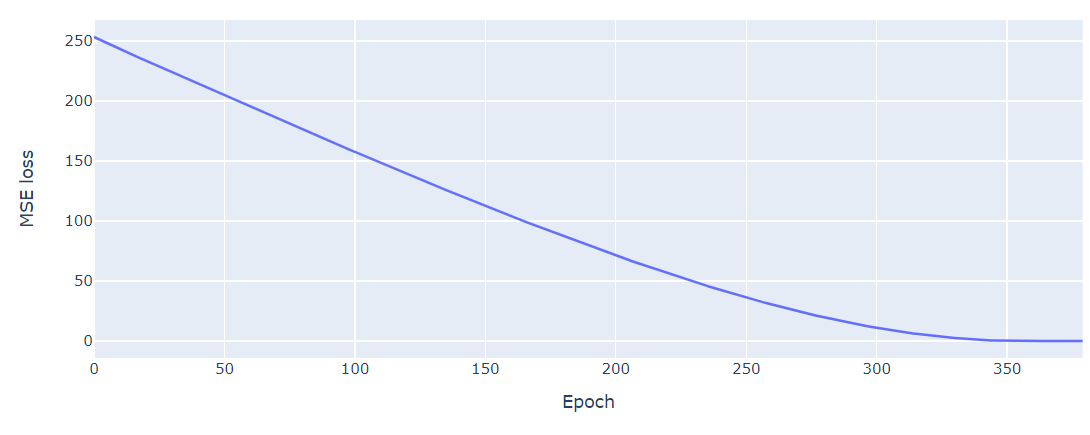
\includegraphics[width=0.8\textwidth]{images/chukotka_train_loss.png}
	\caption{MSE-loss в процессе обучения для Чуктоского АО}
	\label{fig:chukotka_train_score}
\end{figure}

\begin{figure}[h!]
	\centering
	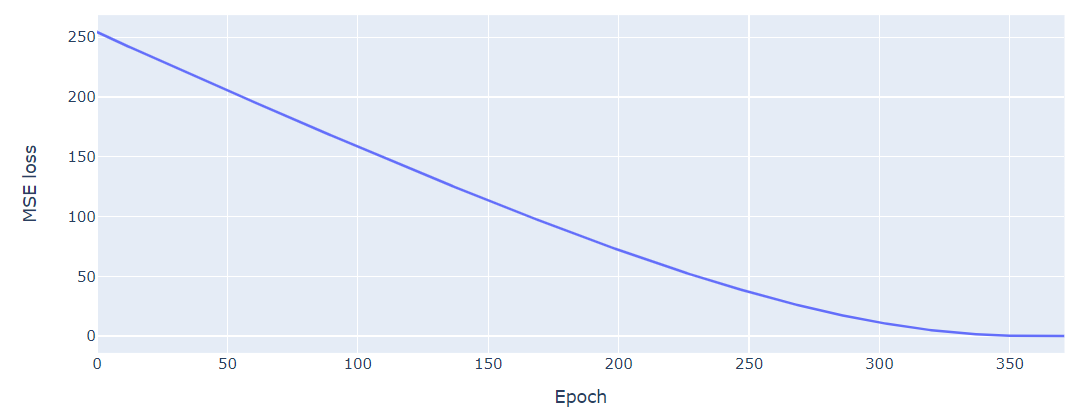
\includegraphics[width=0.8\textwidth]{images/sverdlovsk_train_loss}
	\caption{MSE-loss в процессе обучения для Свердловской области}
	\label{fig:sverdlovk_train_score}
\end{figure}

\begin{figure}[h!]
	\centering
	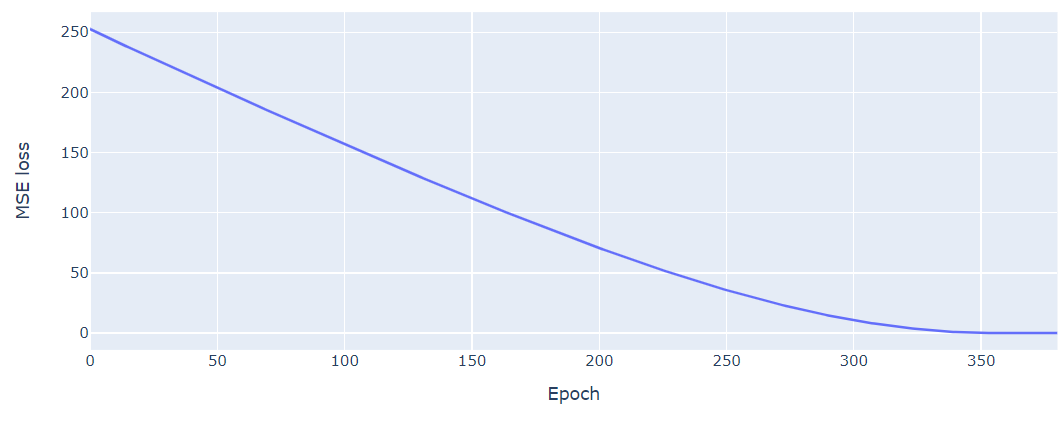
\includegraphics[width=0.8\textwidth]{images/tomsk_train_loss.png}
	\caption{MSE-loss в процессе обучения для Томской области}
	\label{fig:tomsk_train_score}
\end{figure}

Как видно из рисунков \ref{fig:chukotka_train_score}, \ref{fig:sverdlovk_train_score}, \ref{fig:tomsk_train_score}, в процессе обучения нейросеть смогла успешно минимизировать MSE-loss для всех трех областей, для этого потребовалось порядка 350 эпох.

Проиллюстрируем также предсказания, полученные с помощью всех методов, для каждой из выбранных областей.


\begin{figure}[ht]
	\centering
	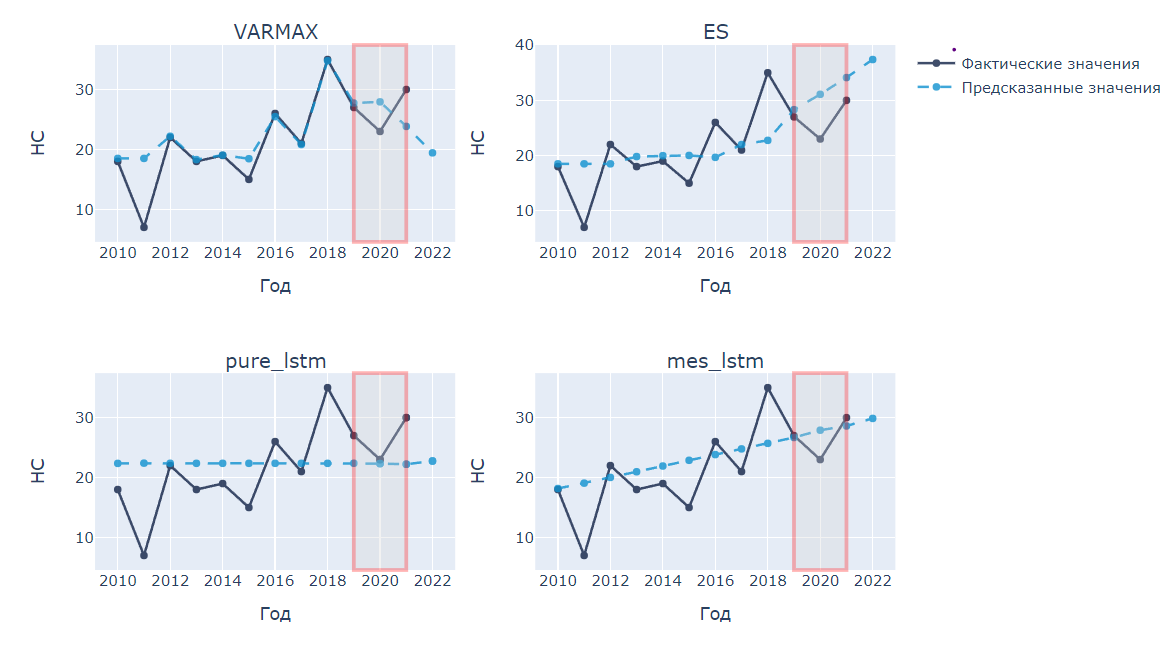
\includegraphics[width=1\textwidth]{images/chukotka_predict.png}
	\caption{Полученные предсказания для Чукотского АО}
	\label{fig:chukotka_predict}
\end{figure}

\begin{figure}[ht]
	\centering
	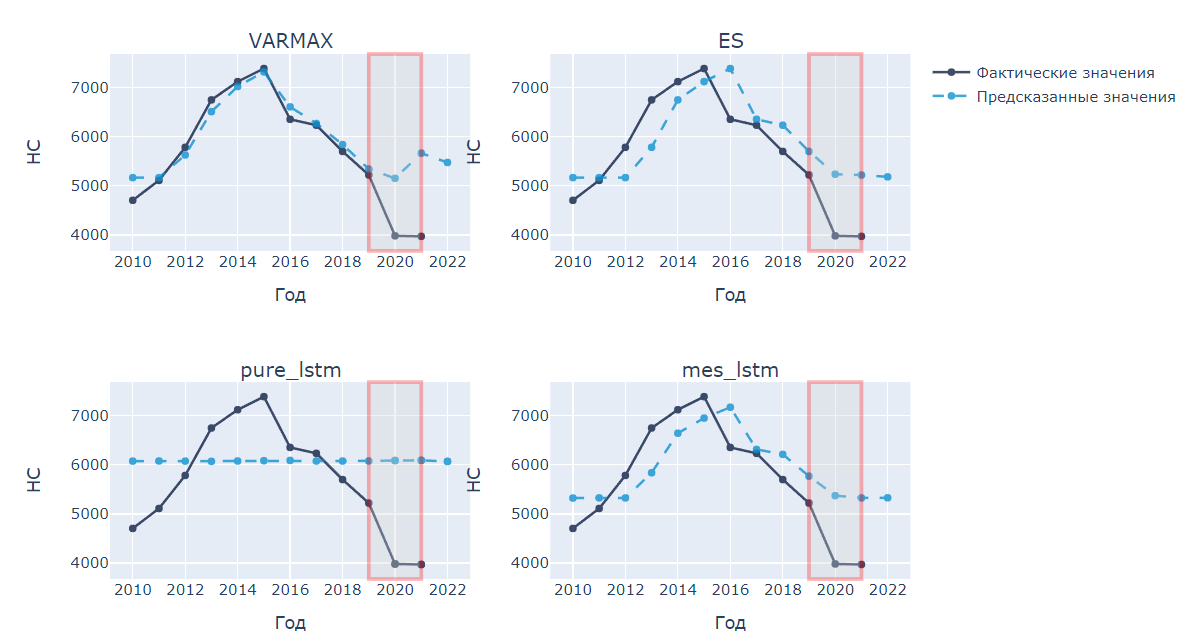
\includegraphics[width=1\textwidth]{images/sverdlovsk_predict.png}
	\caption{Полученные предсказания для Свердловской области}
	\label{fig:sverdlovsk_predict}
\end{figure}

\begin{figure}[ht]
	\centering
	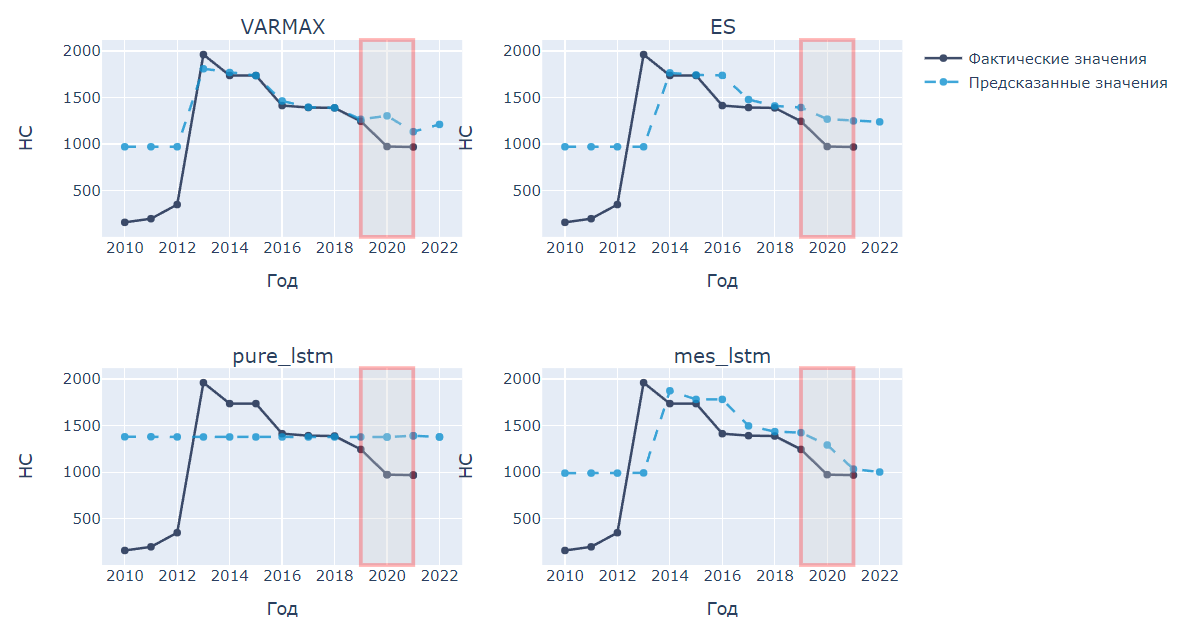
\includegraphics[width=1\textwidth]{images/tomsk_predict.png}
	\caption{Полученные предсказания для Томской области}
	\label{fig:tomsk_predict}
\end{figure}

Как видно из рисунков \ref{fig:chukotka_predict}, \ref{fig:sverdlovsk_predict}, \ref{fig:tomsk_predict}, все модели, кроме LSTM-нейросети в чистом виде, следуют за локальными трендами и строят разумные предсказания. LSTM в чистом виде, по всей видимости, не обучается должным образом, предсказывая каждый раз среднее значение по всему временному ряду. 

Приведем полученные на тестовом множестве и усредненные по субъектам Российской Федерации значения метрик для каждой из обученных моделей на рисунках \ref{fig:covmetric}, \ref{fig:mapemetric}, \ref{fig:rmsemetric}.

\begin{figure}[th]
	\centering
	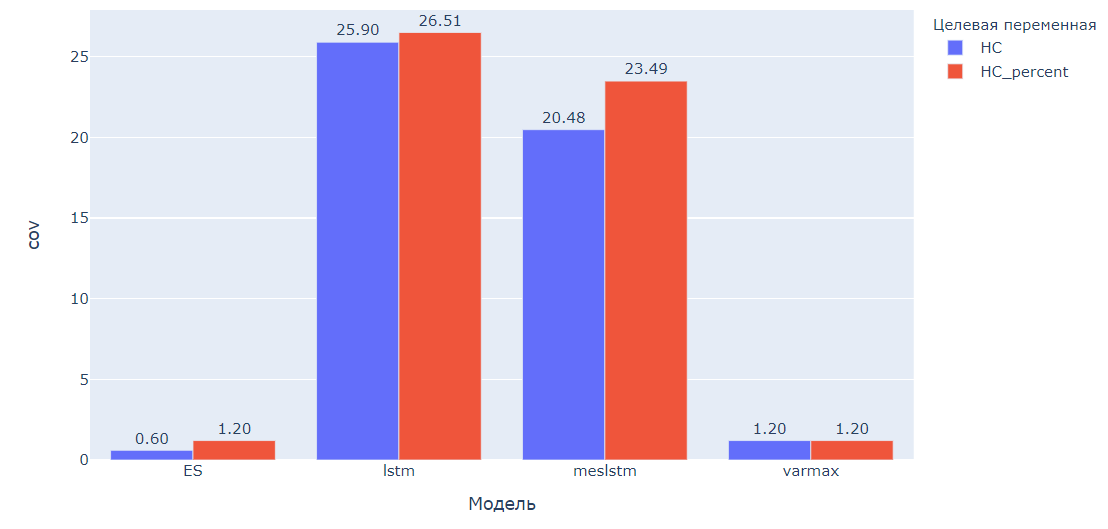
\includegraphics[width=1\textwidth]{images/cov_metric}
	\caption{Усредненное значение метрики COV для всех субъектов по каждой из моделей}
	\label{fig:covmetric}
\end{figure}

\begin{figure}[th]
	\centering
	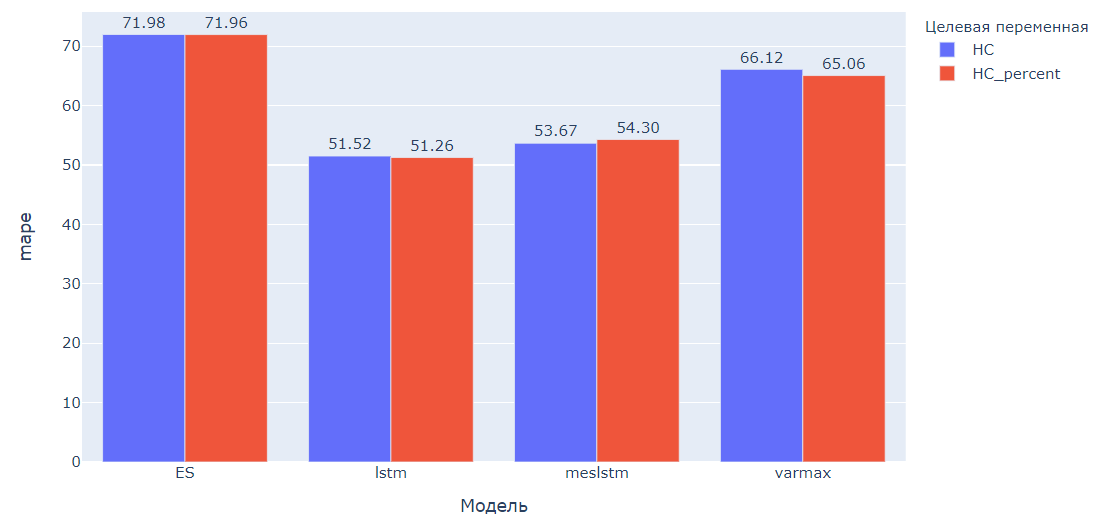
\includegraphics[width=1\textwidth]{images/mape_metric.png}
	\caption{Усредненное значение метрики MAPE для всех субъектов по каждой из моделей}
	\label{fig:mapemetric}
\end{figure}

\begin{figure}[th]
	\centering
	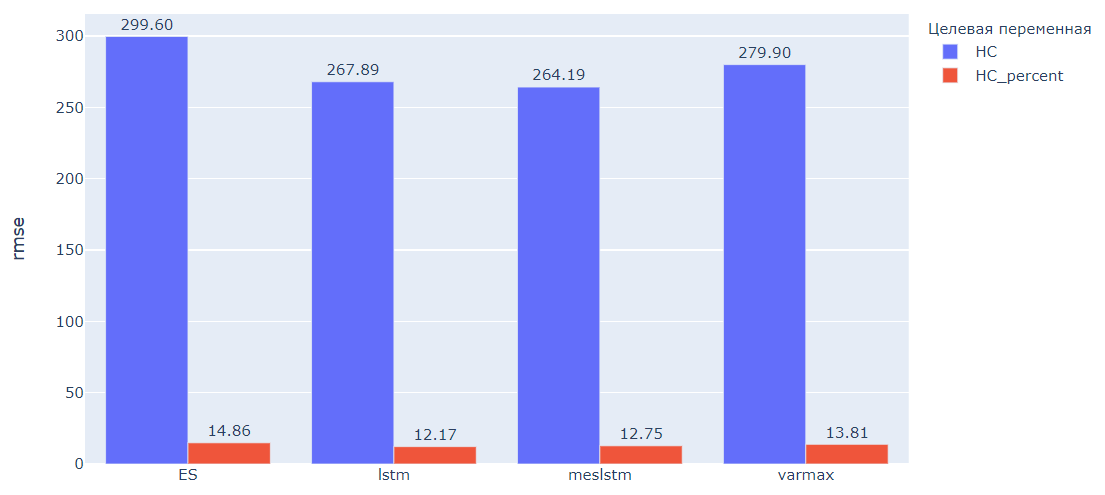
\includegraphics[width=1\textwidth]{images/rmse_metri}
	\caption{Усредненное значение метрики RMSE для всех субъектов по каждой из моделей}
	\label{fig:rmsemetric}
\end{figure}

Судя по приведенным значениям метрик, самой точной моделью оказалась нейросеть LSTM без использования экспоненциального сглаживания, сравнимый результат показала гибридная модель MES-LSTM. Модели VARMAX и ES показали худшее качество на всех метриках.

Таким образом, применение рекуррентной нейросети с использованием дополнительных социально-демографических факторов в нашей задаче позволило превзойти результаты классических статистических моделей. При этом, несмотря на формальное превосходство обыкновенной LSTM, для финального прогноза была выбрана гибридная модель MES-LSTM, как показавшая более разумный подход к предсказанию заболеваемости по результатам предсказаний для Свердловской и Томской областей, Чукотского автономного округа. 

\section{Полученный прогноз}

Модель, показавшая наибольшую точность, была использована для предсказания заболеваемости на 2022 год, с использованием наиболее актуальных данных. Полученные результаты приведены в  таблице \ref{tab:best_prediction}.

% Please add the following required packages to your document preamble:
% \usepackage{graphicx}
% \usepackage{lscape}
\begin{landscape}
	\begin{table}[]
		\caption{Предсказание лучшей модели на 2022 год}
		\label{tab:best_prediction}
		\resizebox{1.5\textwidth}{!} &
				\textbf{Территория} &
				\textbf{НС} &
				\textbf{HC\%} &
				\textbf{Территория} &
				\textbf{НС} &
				\textbf{HC\%} \\ \hline
				г. Санкт-Петербург                & 2510.0 & 48.10  & Ямало-Ненецкий АО               & 198.0  & 35.98  & Оренбургская область         & 1905.0 & 98.98  \\
				Республика Саха (Якутия)          & 165.0  & 16.80  & Московская область              & 3522.0 & 45.35  & Смоленская область           & 320.0  & 33.24  \\
				Чукотский АО                      & 30.0   & 59.12  & Брянская область                & 297.0  & 25.42  & Чеченская Республика         & 151.0  & 12.30  \\
				Республика Северная Осетия-Алания & 194.0  & 27.75  & Республика Татарстан            & 1117.0 & 28.78  & Ивановская область           & 540.0  & 52.94  \\
				Тульская область                  & 634.0  & 41.01  & Владимирская область            & 630.0  & 47.57  & Ленинградская область        & 1403.0 & 77.10  \\
				Новгородская область              & 393.0  & 64.50  & Астраханская область            & 220.0  & 22.43  & Республика Ингушетия         & 60.0   & 10.98  \\
				Липецкая область                  & 292.0  & 26.70  & Саратовская область             & 1134.0 & 46.19  & Омская область               & 1270.0 & 67.71  \\
				Сахалинская область               & 191.0  & 39.21  & Белгородская область            & 225.0  & 14.68  & Республика Калмыкия          & 24.0   & 8.75   \\
				Республика Коми                   & 445.0  & 55.96  & Республика Тыва                 & 48.0   & 14.56  & Еврейская автономная область & 51.0   & 32.70  \\
				Вологодская область               & 359.0  & 31.56  & Нижегородская область           & 1842.0 & 59.17  & Республика Карелия           & 260.0  & 34.11  \\
				Волгоградская область             & 821.0  & 31.59  & Карачаево-Черкесская Республика & 75.0   & 16.26  & Удмуртская Республика        & 1026.0 & 68.73  \\
				Свердловская область              & 5328.0 & 123.68 & Республика Адыгея               & 114.0  & 23.90  & Забайкальский край           & 432.0  & 42.63  \\
				Чувашская Республика              & 338.0  & 27.57  & Тамбовская область              & 223.0  & 21.83  & Иркутская область            & 2752.0 & 113.83 \\
				Республика Марий Эл               & 253.0  & 37.88  & Кемеровская область             & 4566.0 & 167.91 & Челябинская область          & 2978.0 & 86.44  \\
				г. Москва                         & 6843.0 & 54.21  & Курганская область              & 692.0  & 79.42  & Ставропольский край          & 661.0  & 23.04  \\
				Магаданская область               & 49.0   & 35.87  & Орловская область               & 209.0  & 29.22  & Калининградская область      & 451.0  & 44.89  \\
				Республика Мордовия               & 125.0  & 16.19  & Республика Алтай                & 89.0   & 39.96  & Томская область              & 1002.0 & 93.61  \\
				Новосибирская область             & 2854.0 & 106.82 & Камчатский край                 & 149.0  & 48.04  & Калужская область            & 344.0  & 34.18  \\
				Воронежская область               & 635.0  & 27.55  & Ханты-Мансийский АО-Югра        & 1203.0 & 78.67  & Республика Башкортостан      & 2260.0 & 55.93  \\
				Ярославская область               & 524.0  & 41.43  & Псковская область               & 158.0  & 25.76  & Курская область              & 242.0  & 22.42  \\
				Ростовская область                & 1630.0 & 38.74  & Пермский край                   & 2559.0 & 95.40  & Республика Бурятия           & 588.0  & 59.89  \\
				Мурманская область                & 394.0  & 51.61  & Тверская область                & 724.0  & 57.63  & Республика Дагестан          & 419.0  & 12.63  \\
				Архангельская область без АО &
				321.0 &
				30.10 &
				Красноярский край &
				2730.0 &
				95.69 &
				Кабардино-Балкарская Республика &
				250.0 &
				28.80 \\
				Амурская область                  & 212.0  & 27.30  & Краснодарский край              & 2343.0 & 40.83  &                              &        &        \\
				Самарская область                 & 3492.0 & 109.01 & Пензенская область              & 405.0  & 31.87  &                              &        &        \\
				Ненецкий АО                       & 12.0   & 26.47  & Ульяновская область             & 902.0  & 70.91  &                              &        &        \\
				Алтайский край                    & 2182.0 & 100.54 & Кировская область               & 153.0  & 12.14  &                              &        &        \\
				Рязанская область                 & 252.0  & 23.17  & Приморский край                 & 959.0  & 51.14  &                              &        &        \\
				Тюменская область без АО          & 1174.0 & 90.25  & Хабаровский край                & 375.0  & 28.83  &                              &        &        \\
				Республика Хакасия                & 317.0  & 60.09  & Костромская область             & 240.0  & 38.76  &                              &        &        \\ \hline
			\end{tabular}%
		}
	\end{table}
\end{landscape}



\endinput